\documentclass{beamer}
\usepackage[utf8]{inputenc}
\usepackage[spanish]{babel}
\usepackage{amsmath, amsthm, amssymb}
\usepackage{enumitem}
\usepackage{graphicx,caption}

\setitemize{label=\usebeamerfont*{itemize item}%
  \usebeamercolor[fg]{itemize item}
  \usebeamertemplate{itemize item}}

\usepackage[absolute,overlay]{textpos}
  \setlength{\TPHorizModule}{1cm}
  \setlength{\TPVertModule}{1cm}

\AtBeginSection[]
{
  \begin{frame}{Tabla de contenido}
    \tableofcontents[currentsection]
  \end{frame}
}
\beamertemplatenavigationsymbolsempty
\setbeamertemplate{footline}[frame number]

\title{Tamaño máximo de una thrackle de triángulos}
\author [Santiago León O.] {Santiago León Ortiz\\ {\small Asesora: Dra. Dolores Lara Cuevas}}
\institute [Cinvestav, Computación] { }

\usetheme{Madrid}
\begin{document}
\begin{frame}
  \raisebox{-1cm}{%
    \parbox[c]{3cm}{\centering%
      
\includegraphics[width=2cm]{cinvestavlogo.png}%
    }%
    \parbox[c]{\dimexpr\paperwidth-3cm\relax}{\centering%
      {\Large Departamento de Computación\\ Cinvestav Zacatenco}%
    }%
  }%
  \maketitle
\end{frame}

\begin{frame}[allowframebreaks]
  \frametitle{Definiciones}
  \begin{block}{\textit{Intersección de triángulos}}
    Dos triángulos con vértices en un conjunto de puntos, sin aristas en común,
    se \emph{intersectan}, si tienen un vértice en común, o sus aristas se
    cruzan.
  \end{block}
  \begin{figure}[htb]
    \centering
    \input{interseccion_triangulos.pdf_tex}
  \end{figure}
  \begin{block}{\textit{Thrackle de triángulos}}
    Es un conjunto $T$ de $k$ triángulos dibujados sobre un conjunto de
    puntos que cumple las siguientes propiedades:
    \begin{enumerate}
      \item Los triángulos en $T$ no tienen ninguna arista en común.
      \item Cualesquiera dos triángulos en $T$ se intersectan.
    \end{enumerate}
    El valor $k$ es el tamaño del thrackle $T$.
  \end{block}
  \begin{figure}[htb]
    \centering
    \input{thrackle.pdf_tex}
  \end{figure}
\end{frame}

\begin{frame}
  \frametitle{Problema}
  \begin{block}{}
    ¿Cuál es el tamaño máximo de un thrackle de triángulos sobre
    cualquier conjunto de $n$ puntos?
    \begin{itemize}
      \item Se cree que debe ser menor a $\frac{n^2}{9}+2$ triángulos.
    \end{itemize}
  \end{block}
  \begin{columns}
    \begin{column}{0.5\textwidth}
      \begin{center}
        \begin{figure}[htb]
          \centering
          \def\svgwidth{4.5cm}
          \input{n_8_ot_3017_ts_693866964.pdf_tex}
        \end{figure}
      Posición general
      \end{center}
    \end{column}
    \begin{column}{0.5\textwidth}
      \begin{center}
      \begin{figure}[htb]
        \centering
        \def\svgwidth{4.5cm}
        \input{n_8_ot_0.pdf_tex}
      \end{figure}
      Posición convexa
      \end{center}
    \end{column}
  \end{columns}
\end{frame}

\begin{frame}
  \frametitle{Origen del problema}
  \begin{figure}[htb]
    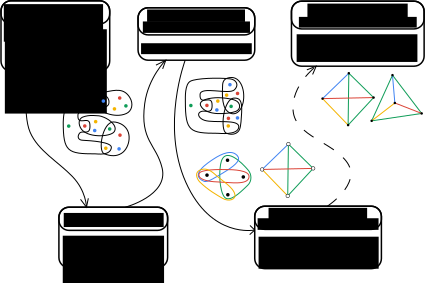
\includegraphics{origen_problema.pdf}
  \end{figure}
\end{frame}

\begin{frame}
  \frametitle{¿Qué se sabe hasta ahora?, cota inferior}
  Cualquier conjunto de $n$ puntos tiene al menos $\lceil\frac{n^2}{12}\rceil$ triángulos
  disjuntos en aristas que contienen al mismo punto en su interior.
  \begin{figure}[htb]
    \def\svgwidth{3cm}
    \input{triangulos_punto_interior.pdf_tex}
  \end{figure}
  \begin{itemize}[leftmargin=2cm]
    \item[$\implies$] Para todo conjunto de $n$ puntos en posición convexa, siempre existe un
      thrackle con $\lceil\frac{n^2}{12}\rceil$ triángulos.
  \end{itemize}
  Si $3|n$ entonces existe un thrackle con $\frac{n^2}{9}+1$ triángulos.
  \begin{itemize}[leftmargin=1cm]
    \item ¿Se cumple para todo $n$?
  \end{itemize}
\end{frame}

\begin{frame}
  \frametitle{¿Qué se sabe hasta ahora?, cota superior}
  Caracterización de los segmentos restantes en un conjunto de triángulos
  disjuntos en aristas de tamaño máximo.
  \begin{figure}[htb]
    \scriptsize
    \input{hanani.pdf_tex}
  \end{figure}
  Un thrackle puede tener máximo $\frac{n^2}{6}-O(n)$ triángulos.
\end{frame}

\begin{frame}[c]
  \begin{center}
    \Huge Resultados: Puntos en posición general.
  \end{center}
\end{frame}

\begin{frame}
  \frametitle{Posición general}
  Valor exacto del tamaño máximo de un thrackle $T_n$ en un conjunto de $n$
  puntos para $3\le n\le 7$.
  \begin{columns}
    \hspace{0.7cm}
    \begin{column}{0.6\textwidth}
      \begin{center}
      \begin{figure}[htb]
        \centering
        \input{n_5_pos_general.pdf_tex}
      \end{figure}
      \end{center}
    \end{column}
    \begin{column}{0.2\textwidth}
        \begin{tabular}{| c | c |}
          \hline
          \textbf{$n$} & \textbf{$T_n$} \\ \hline
          3 & 1 \\ \hline 
          4 & 1 \\ \hline
          5 & 2 \\ \hline
          6 & 4 \\ \hline
          7 & 7 \\ \hline
        \end{tabular}
    \end{column}
    \hfill
  \end{columns}
\end{frame}

\begin{frame}
  \frametitle{Posición general, $n=8$}
  Algoritmo de backtracking para determinar que el tamaño máximo de un thrackle
  sobre un conjunto de 8 puntos.
  \begin{itemize}
    \item Por la cota superior debe haber a lo sumo 8 triángulos.
    \item La cota inferior más alta, ignorando que $3\nmid8$ es $\sim8$.
  \end{itemize}
  \vspace{0.3cm}
  El algoritmo busca un thrackle de 8 triángulos para cada conjunto de 8
  puntos.
\end{frame}

\begin{frame}
  \frametitle{Algoritmo de backtracking 1}
  \begin{figure}[htb]
    \includegraphics<1>{alg_1_1.pdf}
    \includegraphics<2>{alg_1_2.pdf}
    \includegraphics<3>{alg_1_3.pdf}
    \includegraphics<4>{alg_1_4.pdf}
    \includegraphics<5>{alg_1_5.pdf}
    \includegraphics<6>{alg_1_6.pdf}
    \includegraphics<7>{alg_1_7.pdf}
    \includegraphics<8>{alg_1_8.pdf}
    \includegraphics<9>{alg_1_9.pdf}
    \includegraphics<10>{alg_1_10.pdf}
    \includegraphics<11>{alg_1_11.pdf}
    \includegraphics<12>{alg_1_12.pdf}
    \includegraphics<13>{alg_1_13.pdf}
  \end{figure}
\end{frame}

\begin{frame}
  \frametitle{Resultados de la ejecución, para $n=8$}
  La ejecución del Algoritmo 1 para cada conjunto de puntos, utilizando un
  procesador Intel Core i7, arrojó los siguientes resultados:
  \begin{itemize}[leftmargin=1cm]
    \item Existe un thrackle de tamaño 8 para cada conjunto de 8 puntos.
      \begin{itemize}[leftmargin=1cm]
        \item[$\implies$] Un thrackle sobre un conjunto de 8 puntos tiene máximo 8 triángulos.
      \end{itemize}
    \item Nodos recorridos: $\sim$7,838.63 en promedio
    \item Tiempo: 1.34 segundos (0.404 ms en promedio)
  \end{itemize}
\end{frame}

\begin{frame}
  \frametitle{Posición general, $n=9$}
  El tamaño máximo de un thrackle debe estar en el intervalo $[9,12]$.
  \vspace{0.3cm}

  Algoritmo 2 es un versión modificada del anterior que explora el árbol
  completamente y almacena el tamaño máximo de los thrackles.
  \vspace{0.3cm}
  \begin{itemize}[leftmargin=1.5cm]
    \item[$\implies$] Un thrackle sobre un conjunto de 9 puntos tiene máximo 10 triángulos.
  \end{itemize}
  \vspace{0.3cm}

  La ejecución tuvo las siguientes características:
  \begin{itemize}[leftmargin=1cm]
    \item Nodos: $\sim2,526,172.5$ nodos en promedio
    \item Tiempo: $\sim9$ horas 57 minutos (225.5 ms en promedio)
    \item Memoria: Máximo $148.8$ MB por conjunto de puntos
  \end{itemize}
\end{frame}

%\begin{frame}
%  \frametitle{Algoritmo de backtracking 2}
%  \begin{figure}[htb]
%    \includegraphics<1>{alg_1_13.pdf}
%  \end{figure}
%\end{frame}

\begin{frame}
  \frametitle{Posición general, $n=10$}
  El tiempo de ejecución del Algoritmo 2 se hace muy grande. El árbol de
  búsqueda para posición convexa tiene las siguientes propiedades:
  \begin{itemize}
    \item Nodos: 305,532,771 nodos
    \item Tiempo: 12.86 segundos
    \item Memoria: 8.87 GB
      \begin{itemize}[leftmargin=1.5cm]
        \item[$\implies$] 5.84 años para explorar todos los conjuntos de puntos.
      \end{itemize}
  \end{itemize}
  \vspace{0.3cm}
  Varias ejecuciones del Algoritmo 1 prueban lo siguiente:
  \begin{itemize}
    \item Todo conjunto de 10 puntos tiene un thrackle con 11 triángulos.
      \begin{itemize}[leftmargin=1cm]
        \item (Ejecución de 35 minutos).
      \end{itemize}
    \item Aproximadamente 79,712 conjuntos de 10 puntos no tienen un thrackle con 12 triángulos.
      \begin{itemize}[leftmargin=1cm]
        \item (Ejecución de 30 horas).
      \end{itemize}
  \end{itemize}
\end{frame}

\begin{frame}
  \frametitle{¿Cuánto tarda el Algoritmo 2?}
  \begin{itemize}
  \item El número de iteraciones es al menos igual al número de thrackles
    distintos.
  \item El peor caso ocurre para el conjunto de puntos con mayor número de
    thrackles distintos.
  \end{itemize}
      \begin{figure}[htb]
        \centering
        \def\svgwidth{10cm}
        \input{2-convex_n_8.pdf_tex}
      \end{figure}
  ¿Son siempre convexos, o 2-convexos?
\end{frame}

\begin{frame}[c]
  \begin{center}
    \Huge Resultados: Puntos en posición convexa.
  \end{center}
\end{frame}

%\begin{figure}[htb]
%  \centering
%  \def\svgwidth{5cm}
%  \input{3_n.pdf_tex}
%  \caption{Thrackle con $\frac{n^2}{9}+1$ triángulos cuando $3|n$.}
%\end{figure}

\begin{frame}[t]
  \frametitle{Construcción para todo $n$}
  Se extendió la cota inferior del tamaño de un thrackle, para incluir los
  casos en que $n\not\equiv0 \pmod3$.

  \begin{figure}[htb]
    \centering
    \begin{textblock}{5}(4,2.4)
      \def\svgwidth{5cm}
      \input{3_n-1.pdf_tex}
    \end{textblock}

    \begin{textblock}{5.5}(0.2,4.8)
      \def\svgwidth{5.5cm}
      \input{3_n-2-impar.pdf_tex}
    \end{textblock}

    \begin{textblock}{5.5}(7,4.8)
      \def\svgwidth{5.5cm}
      \input{3_n-2-par.pdf_tex}
    \end{textblock}
  \end{figure}
  \vspace{5.3cm}
  Para todos los casos el tamaño es menor (pero cercano) a $\frac{n^2}{9}+2$.
\end{frame}

\begin{frame}
  \frametitle{Número de thrackles para posición convexa}
  Determinamos cuántos thrackles distintos tiene un conjunto de $n$ puntos en
  posición convexa.

  Encontramos una cota inferior analítica para este valor cuando $6|n$.\\
  \begin{columns}
    \begin{column}{0.3\textwidth}
      \begin{center}
        \begin{tabular}{| l | c |}
          \hline
          \textbf{n} & \textbf{Thrackles} \\ \hline
          3 & 1 \\ \hline 
          4 & 4 \\ \hline
          5 & 15 \\ \hline
          6 & 30 \\ \hline
          7 & 30 \\ \hline
          8 & 120 \\ \hline
          9 & 3156 \\ \hline
          10 & 47460 \\ \hline
        \end{tabular}
      \end{center}
    \end{column}
    \begin{column}{0.7\textwidth}
      \begin{block}{Cantidad mínima de thrackles}
        Hay al menos
        $$(p(n/3)-p(n/3-1))\frac{(\frac{n}{3})!\cdot6^{\frac{n}{3}-2}\cdot2^{\frac{n}{6}-1}}{(\frac{n}{6})!\binom{n/3}{2}}$$
        thrackles de triángulos distintos, para $n$ puntos en posición
        convexa con $6|n$. Donde $p(n)$ es el número de formas de sumar $n$
        (función de partición).
      \end{block}
    \end{column}
  \end{columns}
\end{frame}

\begin{frame}
  \frametitle{Orden de triángulos en posición convexa}
  El Algoritmo 1 tiene mejor tiempo de ejecución si ordenamos los triángulos.
  \begin{figure}[htb]
    \centering
    \input{orden_triangulos.pdf_tex}
  \end{figure}
\end{frame}

\begin{frame}
  \frametitle{Orden de triángulos en posición convexa}
  El Algoritmo 1 tiene mejor tiempo de ejecución si ordenamos los triángulos.
  \begin{figure}[htb]
    \centering
    \input{orden_triangulos_1.pdf_tex}
  \end{figure}
\end{frame}

\begin{frame}
  \frametitle{Conclusiones y trabajo futuro}
  \begin{itemize}
    \item Encontramos evidencia para creer que el tamaño máximo de un thrackle
      de triángulos es a lo sumo el valor conjeturado de $\frac{n^2}{9}+2$.
    \item La complejidad computacional de una búsqueda exhaustiva crece bastante
      rápido.
    \item Los conjuntos de 8 y 9 puntos con mayor número de thrackles de tamaño
      máximo son el conjunto en posición convexa o conjuntos de puntos
      2-convexos.
      \begin{itemize}
        \item ¿Es esto cierto para todo $n$?
      \end{itemize}
    \item El orden de los triángulos en posición convexa reduce
      significativamente el tiempo de ejecución.
      \begin{itemize}
        \item ¿Se puede generalizar esta idea a posición general?
      \end{itemize}
  \end{itemize}
\end{frame}

\begin{frame}[c]
  \begin{center}
    \Huge ¡Gracias!
  \end{center}
\end{frame}

\end{document}
